\documentclass[a4paper,12pt,twoside,openright]{report}
\usepackage[titletoc]{appendix}
\usepackage{textcomp}
\usepackage[pdftex]{color,graphics}
\usepackage{amssymb}
\usepackage{verbatim}
\usepackage{graphicx}
\usepackage{graphics}
\usepackage{amsmath}
\usepackage{rotating}
\usepackage{setspace}
\usepackage{multirow}
\usepackage{array}
\usepackage{hhline}
\usepackage[labelfont={bf}, margin=0.5cm]{caption}
\usepackage{pdflscape}
\usepackage{subcaption}
\usepackage{caption}
\usepackage{xspace}
\usepackage{float}
\usepackage{placeins}
\usepackage{etoolbox}
\usepackage{xkeyval}[2006/11/18]
\usepackage{datetime}
\usepackage[a4paper,inner=2.5cm,outer=1.5cm,top=2.5cm,bottom=2.5cm,pdftex]{geometry}
\usepackage{emptypage}
\usepackage{hyperref}

\hypersetup{
	linktocpage,
    colorlinks = true,
	linkcolor = blue,
	citecolor = green
}

\usepackage{fancyhdr}
\fancyfoot{}
\pagestyle{fancy}
\fancyhead[LO]{\leftmark}
\fancyhead[RE]{\rightmark}
\fancyhead[RO,LE]{\thepage}

\renewcommand{\textfraction}{.05}
\renewcommand{\floatpagefraction}{.40}

\newcommand{\gr}{$\gamma$-ray\xspace}
\newcommand{\grs}{$\gamma$-rays\xspace}

\usepackage{lipsum}% just to automatically generate text

\makeatletter
\newcommand\ackname{Acknowledgements}
\if@titlepage
  \newenvironment{acknowledgements}{%
      \titlepage
      \null\vfil
      \@beginparpenalty\@lowpenalty
      \begin{center}%
        \bfseries \ackname
        \@endparpenalty\@M
      \end{center}}%
     {\par\vfil\null\endtitlepage}
\else
  \newenvironment{acknowledgements}{%
      \if@twocolumn
        \section*{\abstractname}%
      \else
        \small
        \begin{center}%
          {\bfseries \ackname\vspace{-.5em}\vspace{\z@}}%
        \end{center}%
        \quotation
      \fi}
      {\if@twocolumn\else\endquotation\fi}
\fi
\makeatother

\newdateformat{monthyeardate}{%
  \monthname[\THEMONTH], \THEYEAR}

%\textheight 24cm
%\textwidth 16.5cm
%\topmargin -1cm
%\oddsidemargin  0cm
%\evensidemargin 0cm
%\flushbottom

%\usepackage{etoolbox}
%\patchcmd{\chapter}{\thispagestyle{plain}}{\thispagestyle{fancy}}{}{}

\setlength{\headheight}{15pt}


\begin{document}


\setcounter{secnumdepth}{3}
\setcounter{tocdepth}{3}

%\doublespace

\pagenumbering{roman}

\begin{titlepage}

\begin{center}

\textbf{\Huge Upgrades to the }

\vspace{3mm}

\textbf{\Huge Fluorescence Detectors of the}

\vspace{3mm}

\textbf{\Huge Pierre Auger Observatory} 

\vspace{3cm}


\includegraphics[width=0.3\textwidth]{pix/UoA_col_vert.png}

\vspace{3cm}


\textbf{\large Tristan William Sudholz} \\
\vspace{0.4cm}
\large School of Physical Sciences \\
\vspace{0.1cm}
\large University of Adelaide

\vspace{1.5cm}
\large This dissertation is submitted for the degree of \\
\vspace{0.2cm}
\textit{\large Doctor of Philosophy}
\vspace{2.5cm}

\monthyeardate\today

\end{center}

\end{titlepage}

%\chapter*{Declaration}

I, Tristan William Sudholz, certify that this work contains no material which has been accepted for the award of any other 
degree or diploma in any university or other tertiary institution and, to the best of my knowledge and
belief, contains no material previously published or written by another person, except where due
reference has been made in the text. In addition, I certify that no part of this work will, in the future,
be used in a submission for any other degree or diploma in any university or other tertiary institution 
without the prior approval of the University of Adelaide and where applicable, any partner institution
responsible for the joint-award of this degree.

I give consent to this copy of my thesis, when deposited in the University Library, being made
available for loan and photocopying, subject to the provisions of the Copyright Act 1968.

I also give permission for the digital version of my thesis to be made available on the web, via the
University’s digital research repository, the Library catalogue and also through web search engines,
unless permission has been granted by the University to restrict access for a period of time. 

\vspace{2cm}

\line(1,0){150}

\vspace{1cm}

Tristan William Sudholz
\chapter*{Abstract}


%
\chapter*{Acknowledgements}



\tableofcontents
%\listoffigures
%\listoftables

\chapter*{Nomenclature}

\addcontentsline{toc}{chapter}{Nomenclature}

\begin{tabular}{p{8em} p{30em}}
PAO & Pierre Auger Observatory \\
EAS & Extensive Air Shower \\
NSB & Night Sky Background \\
PE & Photo-electron \\
FD & Fluorescence Detector \\
SD & Surface Detector \\
PMT & Photomultiplier Tube \\
FLT & First Level Trigger
\end{tabular}

\chapter*{Introduction}\label{Ch:Intro}
\markright{Introduction}
\addcontentsline{toc}{chapter}{Introduction}
\pagenumbering{arabic}

\begin{itemize}
\item Define Cosmics Rays.
\item The origins of the highest energy cosmic-rays still unknown.
\item First detection by Pierre Auger in 1937 and the current detector looking at theses energies is the Pierre Auger Observatory.
\item Hybrid experiment containing both surface detectors and fluorescence detectors
\item Surface detector has nearly 100\% up-time while the fluorescence detectors only have 15\% up-time.
\item **** Proposal to extend the fluorescence detector up-time. To achieve this will have to operator while the moon is above the horizon. This will increase the level NSB and will have the PMTs run under a reduced gain to compensate. ****
\item Photomultiplier Tubes are used as pixels within the camera of the fluorescence detectors and  the aim of these thesis is to quantify the characteristics of the PMT under the reduced gain and increased.
\item Outline a Summary of each chapter.
\end{itemize}


Cosmic-rays are particles that originate outside of the Earth atmosphere. These particles can be photons, hadronic or leptonic in nature [ref?]. In this thesis, when mentioning cosmic-rays I will mean the hadronic component unless specified otherwise. Cosmic-rays have been measurement over a large range of energies (over 6 decades in energy) and it has many interesting features have been observed in this energy spectrum. One of the longest running mysteries is what happens at the highest energy. Since the first detection of extensive air showers by Pierre Auger in 1937 [ref], many different experiments have endeavoured to solve this mystery. The Pierre Auger Observatory [ref] is currently in operation to observe cosmic-rays at the highest energies. 

The Pierre Auger Observatory is a hybrid experiment consisting of both surface detectors and fluorescence detectors. (Outline location) The surface detector has a nearly 100\% operation up-time {ref} while the fluorescence detectors only 15\% operation up-time [ref]. (Outline how PAO detects cosmic-rays, just need a brief summary).

A current proposal to extend the fluorescence detector operation up-time. Extended up-time would be beneficial as the fluorescence detectors image the entire extensive air shower and would increase the number of showers observed through out yearly observation. To achieve the extended operation the fluorescence detectors would have to operated while the moon is above the horizon. While the moon is up, this would increased the Night Sky Background level and to compensate the Photomultiplier Tubes acting as the camera pixels would have to be run under reduced gain. 

The aim of this thesis is to quantify the characteristics of the Photomultiplier Tubes operating under this reduced gain and outline any operation strategies. Outline of each chapter is as follows:

\begin{itemize}
\item  Chapter \ref{Ch:Cosmic-rays}: Cosmic-rays

Does this work as a new line

\item Chapter \ref{Ch:CR_Detection}: Detection of Cosmic-Rays

Add text here

\item Chapter \ref{Ch:PAO}: The Pierre Auger Observatory

Add text here

\item Chapter \ref{Ch:SelectEff} : EAS Selection Efficiency with Increased NSB 

Add text here

\item Chapter \ref{Ch:PMTCharacter} : Quantifying Characteristics of the FD PMT 

Add text here

\item Chapter \ref{Ch:CompSimPMT} : Computer Simulation of the FD PMT 

Add text here

\item Chapter \ref{Ch:GainVariance} : Measuring Gain Variance of the FD PMT with CalA data 

Add text here

\item Chapter \ref{Ch:LabPMTshift} : Laboratory Simulation of FD Shifts

Add text here

\item Chapter \ref{Ch:CloudCuts} : Effectiveness of Cloud Camera Cuts

Add text here

\item Chapter \ref{Ch:Conclusion}: Conclusion 

Future Work


\end{itemize}
\chapter[Cosmic-Rays]{\centering Cosmic-Rays \\}\label{Ch:Cosmic-rays}

\section{History of Cosmic-Rays}

First detection of ionizing radiation. 

1785: Coulomb found that 
electroscopes can spontaneously 
discharge by the action of the air 
and not by defective insulation

1835: Faraday confirms the 
observation by Coulomb, with 
better insulation technology

1879: Crookes measures that the 
speed of discharge of an 
electroscope decreased when 
pressure was reduced 

\section{Energy Spectrum and Mass composition}

\begin{figure}[hp]
\centering
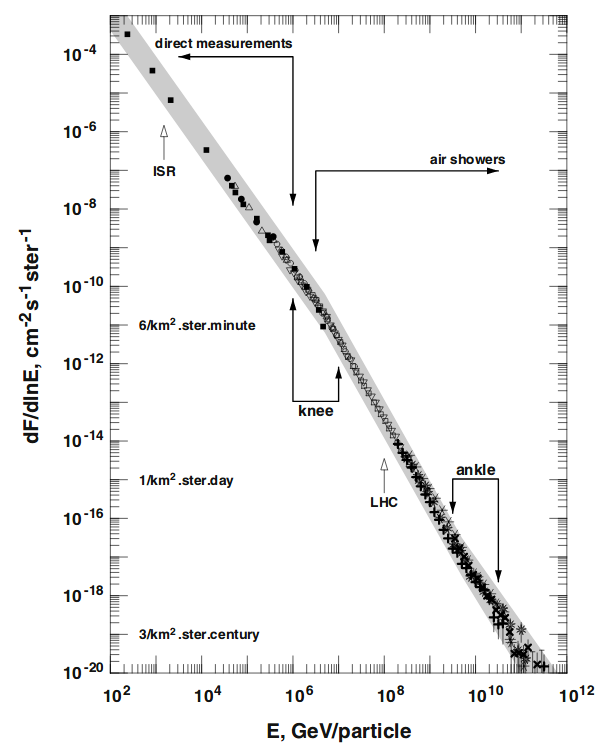
\includegraphics[width=\textwidth]{chapters/pix/CosmicRay_Spectrum.png}
\caption{Measured energy spectrum of cosmic-rays from 100 GeV up to the highest detected energy.}
\label{fig:CR_Spectrum}
\end{figure}

Cosmic-rays have been detected over a large range of energies from GeV (10$^9$ \ eV) to above EeV (10$^18$ \ eV). Spectrum in Figure \ref{fig:CR_Spectrum} shows the break at the knee and ankle and which type of experiments are most suited to measurement each part. Cosmic-ray spectrum starts out at E$^{-2}$ \ and can be as steep as E$^{-2.7}$ at the highest energies.

Cosmic-rays can consist of protons to iron. 

\section{Production Method and Sources}

Supernova explosions 

AGN jets

other energetic processes

dark matter annihilations.
\chapter{Detections of Cosmic-Rays}\label{Ch:CR_Detection}

\section{Extensive Air Showers}

Use Earth's atmosphere as an interaction medium.
Primary particle interacts with the molecules in the atmosphere to produce a cascade of secondary particles. This cascade of particles is referred to as an Extensive Air Shower (EAS).
Hadronic primaries can produce pions, muons and other stuff.
Mixture of a hadronic core with an electromagnetic component from the decay of $\pi^{0}$.

Shower profile has particles produced until energy on individual secondary particles drop below the ionization threshold. Therefore the shower will reach a point of maximum particle number then will drop off.

\section{Fluorescence Production}

The charge particles of EAS interact with the nitrogen molecules in the atmosphere. This interaction turns the nitrogen molecule dipole like and when the nitrogen returns to a ground state, a photon is emitted. This emitted photon is termed fluorescence light. Fluorescence light is can be emitted isotropically and typically in the UV band (between 300 and 400 nm). *** Show wavelength profile ***


\section{Atmospheric Effects}




\section{Detectors and History}

Early Experiments:

Volcano Ranch

Haverah Park

SUGAR

Yakutsk array is located in Russia and has been operating in different forms since 1967. The array reached a maximum collecting area of 17 km$^2$ around 1990. Recently it has been reconfigured to have a collection area of 8 km$^2$ to study lower energy cosmic-rays.

Akeno Gaint Air Shower Array (AGASA) is located in Tokyo, Japan. Operating at an average altitude of 667 m above sea level from 1990 to 2004. The array consist of over one hundred scintillator detectors covering 100 km$^2$ ***check this***. The timing measurements and data collection is achieved via interconnected optical fibers.

The Fly's Eye was the first successful air fluorescence detector operating from 1981 to 1993 at the Dugway Proving Grounds in Utah, USA. Fly's Eye achieved a time averaged aperture of about 100 km$^2$sr at the highest energies, considering it only operated on clear moonless nights. 

HiRes improved on the Fly's Eye design by advancing resolution and sensitivity, This was achieved by increasing the telescope effective mirror area to 3.8 m$^2$ and reducing the camera pixel angular diameter to 1\textdegree. 
\chapter{Pierre Auger Observatory}\label{Ch:PAO}


Science Goals

Location

\section{Hybrid Detector}

\subsection{Surface Detector}

\subsection{Fluorescence Detector}

\section{Communication System and CDAS}

\section{Event Reconstruction}

\subsection{Surface Detector}

\subsection{Fluorescence Detector}

\section{Enhancements and future upgrades}
%\input{chapters/}
%\input{chapters/}
%\input{chapters/}
%\input{chapters/}

\chapter[Conclusion]{\centering Conclusion \\} \label{Ch:Conclusion}
  

\section{Future Work}



\begin{appendices}
%\input{appendix/}
%\input{appendix/}
%\input{appendix/}
%\input{appendix/}
\end{appendices}

\bibliographystyle{IEEtr}
\bibliography{PhD_PaperBiblography}

\end{document}